\section{Numerical Model Considerations}

\subsection{Material Properties}

Acoustic waves are assumed to propagate in an inviscid fluid with small amplitudes of vibration, negligibly density variations and negligibly convective effects. Wave propagation will thus depend only on fluid density $\rho_a$ and its bulk modulus $K_s$. For air, using the relation $c= \sqrt{\frac{K_s}{\rho_0}}$, the values can be specified as follows:
\begin{eqnarray*}
\rho_a & = & 1.18 \text{ kg/m}^3\\
c & = & 343 \text{ m/s} 
\end{eqnarray*}

Moreover, Bandola's plates are made of wood, an orthotropic material which according to the way it was extracted from the tree, could present transverse isotropy. For plates of musical instruments transverse isotropy is common and their material properties are thus specified through five elastic values: Young's modules $E_x$ and $E_y$, Poisson's ratio $\nu_{xy}$, shear modulus $G_{xy}$ and the plate material density $\rho_p$. Although orthotropic properties can be introduced in numerical models, dynamic expressions for plates could be simplified by considering isotropic properties which also simplify numerical computing.\\

The modal analysis proposed in this work is dedicated to study the coupling phenomenon at low resonances, and simple numerical models are pursued in order to ease monitoring the influence of some specific model parameters. The effect of orthotropy over coupling won't be considered as analysis subject, therefore, plates material will be modelled as an isotropic material.\\

For isotropy, elastic values of \textit{Young's Modulus} and \textit{Poisson's ratio} are defined through the geometric mean of properties presented for spruce in \cite{J.Torres1} and rosewood in \cite{Elejabarrieta}. The elastic properties that were used for the average are presented in Table \ref{OrthoMat}. Wood densities are also presented in this table. The averaged values for isotropic plates are presented in Table \ref{IsoMat}.  

\begin{table}[htb]
\centering
\begin{tabular}{|c|c|c|c|c|c|}\hline
\multicolumn{6}{|c|}{\vphantom{\LARGE Ap} Material with transverse isotropy}\\ \hline\hline
 & $\rho_p \quad (\text{kg/m}^3)$ & $E_x$ (GPa) & $E_y$ (GPa) & $\nu_{xy}$ & $G_{xy}$ (GPa)\\ \hline
Top plate (Spruce) & 330 & 0.66 & 6.6 & 0.003 & 0.77 \\ \hline
Back Plate (Rosewood) & 775 & 2.2 & 16 & 0.05 & 1.1 \\ \hline
\end{tabular}
\caption{Elastic properties for material with transverse isotropic}
\label{OrthoMat}
\end{table}

\begin{table}[htb]
\centering
\begin{tabular}{|c|c|c|}\hline
\multicolumn{3}{|c|}{\vphantom{\LARGE Ap} Averaged isotropic material}\\ \hline\hline
 & $E$ (GPa) & $\nu$ \\ \hline
Top plate (Spruce) & 2.08 & 0.01 \\ \hline
Back Plate (Rosewood) & 5.93 & 0.13 \\ \hline
\end{tabular}
\caption{Elastic properties for isotropic material.}
\label{IsoMat}
\end{table}

\subsection{CAD Models and analysis considerations}


\subsubsection{CAD Models}

Figure \ref{PlateDimensions} presents CAD model for top plate which consists of a drop-shaped plane surface, and the dimensions are specified. The back plate has the same shape except that it does not present a hole.

\begin{figure}[h]
\centering
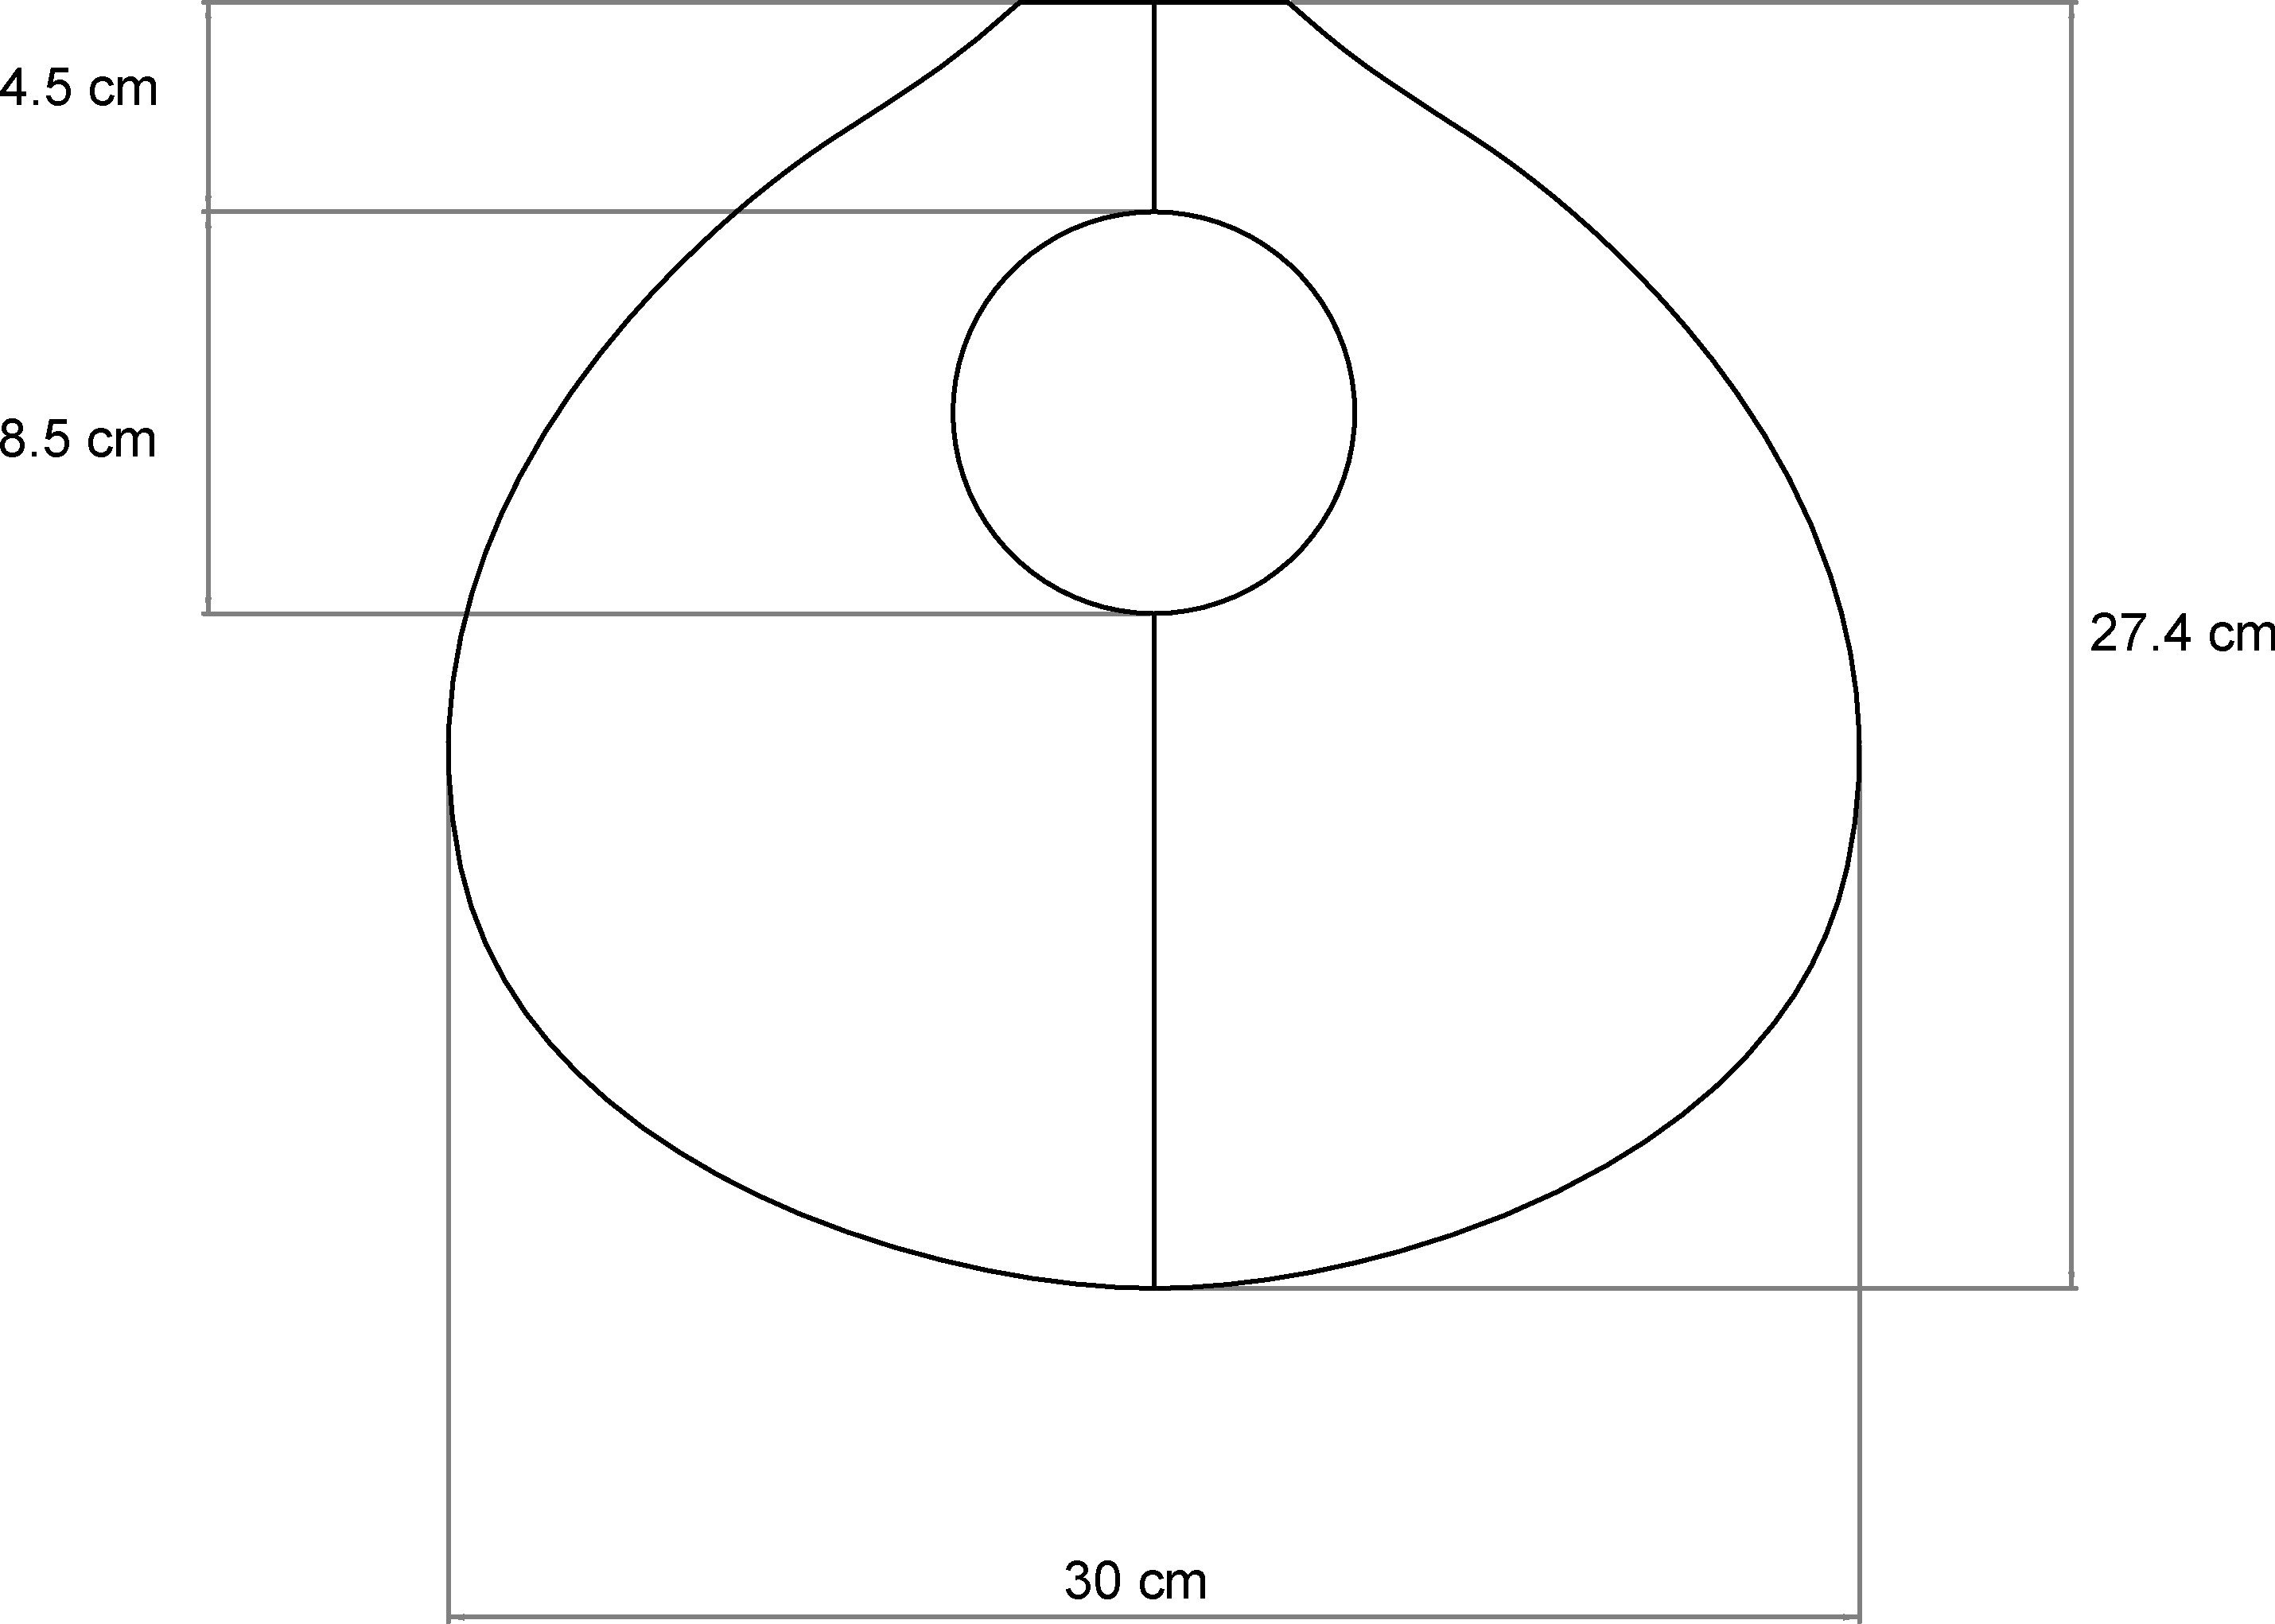
\includegraphics[height=6cm]{img/bandolaFrontarea.pdf}
\caption{Dimensions of modeled plates}
\label{PlateDimensions}
\end{figure}


As it was mentioned, simple models are pursued and hence, fan bracing, harmonic bars, bridge and sound hole reinforcement are not considered. These parts of the bandola, at low resonances, are expected to increase mass and stiffness without changing the shape modes.

It was stated that the air inside the cavity vibrates at the first mode almost as a Helmholtz resonator. This assumption is not so simple because of the geometry of the instrument and also because the cavity walls are not completely rigid. Additionally, the concept of "length of the neck" does not refer exactly to a length determined by either end of the neck. In guitars, for example, it could be thought that the length of the plug of the air is given by top plate thickness, however, practice have shown that an extra volume both inside and outside moves with the air in the neck due to the inertia of the oscillating piston when it gets to its original position. This event is called the \emph{end effect} and the correction that should be applied in order to consider it is related to and of similar size to the diameter of the hole, so the mass of air is substantial. Applying the the correction used for guitars, the effective length of the ``plug" of air of the bandola will be about 1.7 times the radius of the hole.

%which is given by top plate thickness (3mm).
The CAD model of enclosed air should represent the enclosed volume of air together with the effective length of the resonator's neck. The model presented in Figure \ref{CADBody} could represent not only the above ideas, but also the complete body, formed by surface planes for plates and enclosed volume of air, which is useful for coupling the systems. The ribs have a depth of {10 cm} as specified.

\begin{figure}[h]
\centering
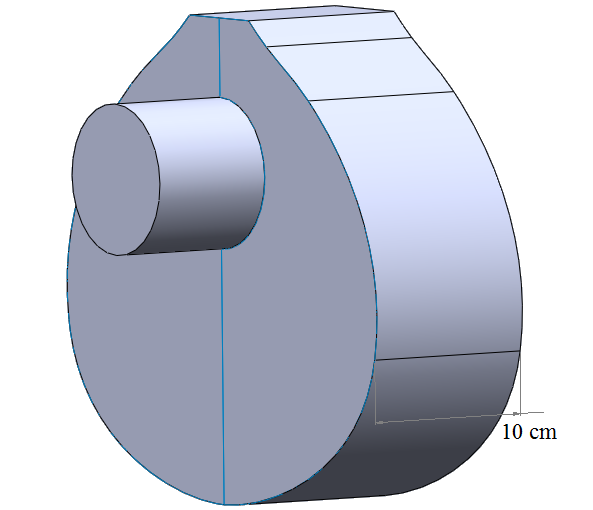
\includegraphics[height=5cm]{img/CADBody.png}
\caption{CAD model for Bandola's resonance box}
\label{CADBody}
\end{figure}

\subsubsection{FEA Considerations}

Simulations were executed using the commercial software ANSYS\textsuperscript{\textregistered} in a range of analysis of {0--800 Hz}, both for separate (top-plate, back-plate, enclosed air) and coupled systems. Boundary conditions are imposed in each case.\\

Separate top and back plates are assumed to vibrate clamped at the edge, i.e., the transverse displacement function and its slope equal to zero. The analysis of plates was performed using the element SHELL281 whose formulation is based on the Mindlin-Reissner theory. For the enclosed air, the pressure at the external transverse area of the sound hole equals the atmospheric pressure. This characteristic allows the air to move in and out the cavity as in a Helmholtz resonator; the walls are considered rigid. The element FLUID220 was used for meshing the air, an element based on governing equation for acoustics, namely the 3-D wave equation, and also takes into account the coupling of acoustic pressure and structural motion at the interface.\\

For the coupled system of top plate-enclosed air, Bandola's top plate and back plate are clamped to the ribs and they enclose the air; back plate is considered rigid but top plate vibration couples the system. The enclosed air has the same boundary conditions as in the separate model but only the top plate moves. The coupling condition is present over the top plate-air interface and states that normal to the interface, fluid particle accelerations are equal to plate accelerations. The coupled system of top plate-enclosed air-back plate has the same conditions presented above but now, back plate can vibrate clamped at the edge and the coupling condition is also specified for back plate-air interface.



